\chapter{Taxonomy}
\label{chap:intro}

In this chapter, we first briefly introduce two existed taxonomies about movement and mobility analysis respectively given by Dodge et al.\cite{dodge2008towards} and Andrienko et al.\cite{andrienko2017visual}. And then we propose our own taxonomy which is an integration of data modeling, techniques and applications. 


\section{Taxonomy by Dodge et al}

Dodge et al.\cite{dodge2008towards} proposed a taxonomy on visualization of movement based on many previous surveys. The taxonomy present a hierarchical structure of the patterns that can be extracted from a variety of movement data, these patterns can be further considered into the mining algorithms design and visualization design, as Figure~\ref{fig:dodgetax} shows:

\textbf{Generic patterns and behavioral patterns:} As the two sub-branches of the root, the generic patterns and behavioral patterns differ in the specificity of the movement. The generic patterns are the low level building blocks, these patterns exist in the general movement data, like the prorogation(traffic congestion, disease) and periodicity(species migration, traffic congestion). The behavioral patterns more focus on patterns under the specific context or for the specific object, like the fighting and foraging. 

\textbf{Primitive and compound patterns:} The generic patterns can be further classified into primitive and compound patterns, according to the number of variable parameters. The primitive patterns is the simplest form of movement with only one changing parameter. On the other hand, the compound patterns involves the changing of multiple parameters. Further more, the Primitive patterns can be classified by the spatial temporal features, which includes spatial patterns, temporal patterns and spatial temporal patterns. While all the compound patterns involve both spatial and temporal features.

Many similar taxonomy also exist, the commonality of them is that all of these work are based on the information that can be extracted from movement data. 

\begin{figure}[!htb]
  \centering
  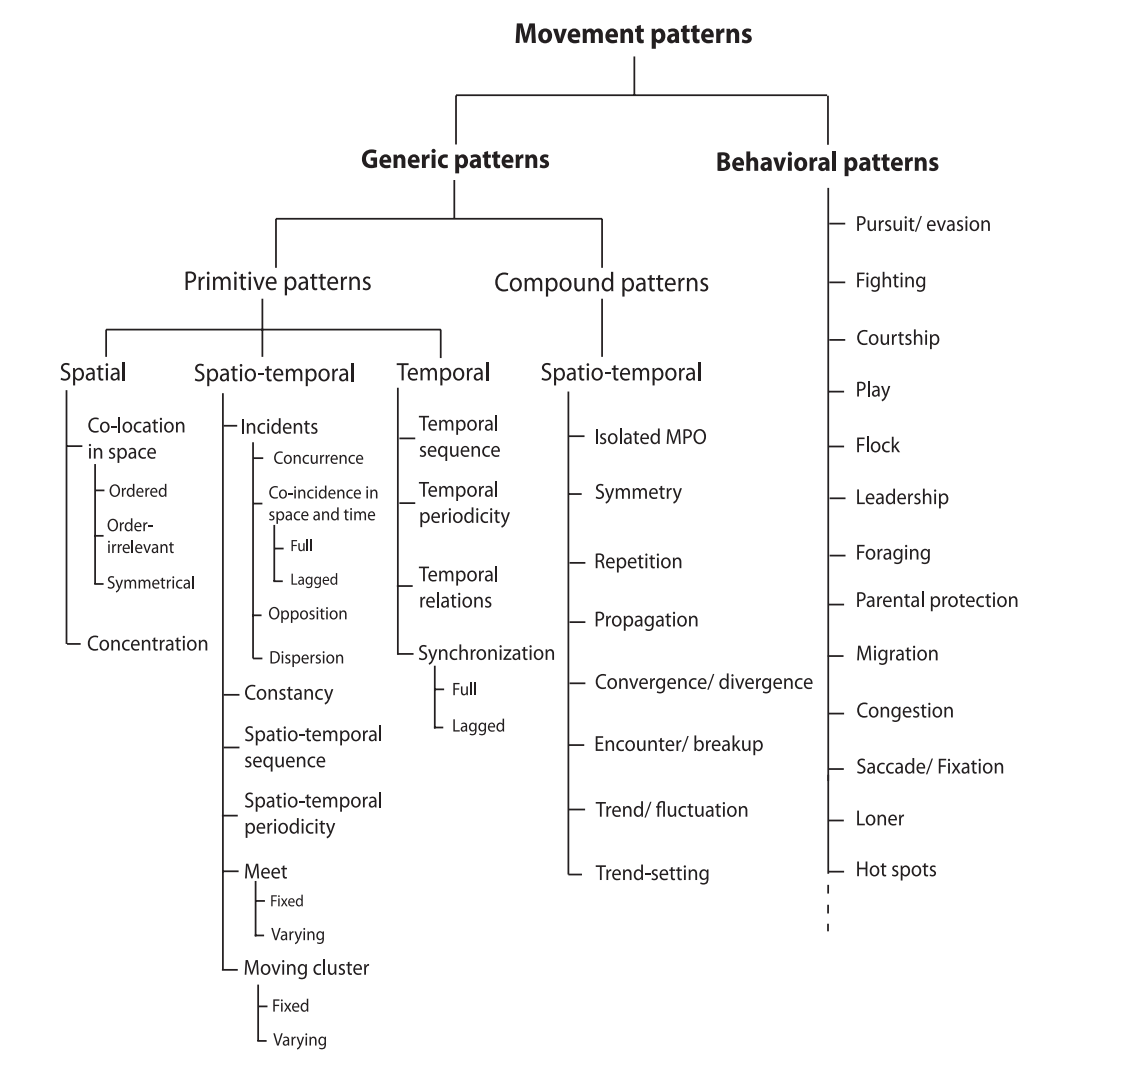
\includegraphics[width = 400px]{figures/dodgetax.png}
  \caption{Dodge's taxonomy of movement patterns.}
  \label{fig:dodgetax}
\end{figure}


\section{Taxonomy by Andrienko et al}
Another category of classification is based on the study object or some high-level application problems. In this section we introduce a recent work from Andrienko et al.\cite{andrienko2017visual}. 

In this survey,the previous work are divided into four large categories: "Data", "Movement and Transportation Infrastructure", "Movement and Behavior", "Modeling and Planning". However, since the "Data" section is an summary of the features and transformations of movement data, which works as fundamental of other sections, we will not list this section into the taxonomy. 

\textbf{Movement and Transportation Infrastructure:} This category focus on the human movements with the transportation infrastructure, including vehicles and pedestrians along the transportation routes, as well as the people through in the public transportation facilities like Subway, bus and train. This category can be further divided into sub-branches including: 

\begin{itemize}
	\item Details of Individual Movements
	\item Variety of Taken Routes
	\item Movement Dynamics Along a Route
	\item Details of Individual Movements
	\item Linking Origins to Destinations
	\item Collective Movement Over a Territory
	\item Events
	\item Contextualizing Movement
	\item Impacts and Risks
\end{itemize}

\textbf{Movement and Behavior:} This category focus on the behavior behind the movement, in addition to the mobility itself, this category more focus on the reasoning of specific movement patterns, like the interest, activities, etc. This category is further divided into three following divisions: 

\begin{itemize}
	\item Use of Transport
	\item Mass Mobility
	\item People’s Activities and Interests
\end{itemize}

\textbf{Modeling and planning:} This category focus on the analytics of traffic modeling and transportation planning. This includes the derivation of models from data, applications of forecasting and simulation, transportation scheduling.

\section{Taxonomy design based on modeling}
Dodge's taxonomy is based on the patterns that can be extracted from the movement data; while Andrienko's taxonomy focuses on the applications. After reviewing the research work in the past tens of years, we have found there are three types data modeling methods, which are spatial points, origin-destination and trajectory. These three modeling methods differ in the granularity of movement and are respectively utilized in different data or applications. 

\modify{taxonomy shouldn't include the interactions and aggregation}

In spatial temporal analysis, aggregation works as a very important step, but the aggregation methods are quite different under different modeling methods. We plan to introduce the aggregation techniques as the start of each subcategory. The overall structure taxonomy is described as follows:

\textbf{Mobility based on spatial points:} In this category, the mobility will be analyzed through the separated spatial points. It should be noted that in this category, the movement of individual mover will not be tracked, the spatial points can reflect the overall spatial distribution of movers, and the distribution of multiple time will indicate the overview movement. We first introduce the aggregation techniques that will be used in the spatial points. Then we classify the previous work based on the entity to be analyzed, including movers and events.

\textbf{Mobility based on origin-destination:} In this category, the movement among origin and destination will be analyzed. We first introduce the aggregation, query and interaction based on origin-destination. Then we classify this category into single origin/destination and multiple origin/destination, which could be further adapted to the different application problem.

\textbf{Mobility based on trajectory:} In the category, the movement records are collected in a finest-grained level and provide a way to conduct the fine-grained tasks, like individual monitoring. In addition to the aggregation techniques and interaction techniques, we further classify the research about trajectory into massive analysis and individual analysis.



